\documentclass[journal=esthag,manuscript=article]{achemso}
%%%%%%%%%%%%%%%%%%%%%%%%%%%%%%%%%%%%%%%%%%%%%%%%%%%%%%%%%%%%%%%%%%%%%
%% Place any additional packages needed here.  Only include packages
%% which are essential, to avoid problems later. Do NOT use any
%% packages which require e-TeX (for example etoolbox): the e-TeX
%% extensions are not currently available on the ACS conversion
%% servers.
%%%%%%%%%%%%%%%%%%%%%%%%%%%%%%%%%%%%%%%%%%%%%%%%%%%%%%%%%%%%%%%%%%%%%
\usepackage[T1]{fontenc}       % Use modern font encodings
\usepackage[utf8]{inputenc}
\usepackage{amsmath}
\usepackage{enumerate}

\usepackage{todonotes}

%%%%%%%%%%%%%%%%%%%%%%%%%%%%%%%%%%%%%%%%%%%%%%%%%%%%%%%%%%%%%%%%%%%%%
%% If issues arise when submitting your manuscript, you may want to
%% un-comment the next line.  This provides information on the
%% version of every file you have used.
%%%%%%%%%%%%%%%%%%%%%%%%%%%%%%%%%%%%%%%%%%%%%%%%%%%%%%%%%%%%%%%%%%%%%
%%\listfiles

%%%%%%%%%%%%%%%%%%%%%%%%%%%%%%%%%%%%%%%%%%%%%%%%%%%%%%%%%%%%%%%%%%%%%
%% Place any additional macros here.  Please use \newcommand* where
%% possible, and avoid layout-changing macros (which are not used
%% when typesetting).
%%%%%%%%%%%%%%%%%%%%%%%%%%%%%%%%%%%%%%%%%%%%%%%%%%%%%%%%%%%%%%%%%%%%%
%% \newcommand*\mycommand[1]{\texttt{\emph{#1}}}


%%%%%%%%%%%%%%%%%%%%%%%%%%%%%%%%%%%%%%%%%%%%%%%%%%%%%%%%%%%%%%%%%%%%%
\author{Eduard Szöcs}
\affiliation[Institute for Environmental Sciences]{Institute for Environmental Sciences, University of Koblenz-Landau, Germany}
\email{szoecs@uni-landau.de}
\phone{+49 (0)6341 280 31552}

\author{Marvin Brinke}
\affiliation[German Federal Institute of Hydrology]{German Federal Institute of Hydrology (BfG), Koblenz, Germany}

\author{Bilgin Karaoglan}
\affiliation[German Federal Environmental Agency]{Federal Environmental Agency (UBA), Dessau-Roßlau, Germany}

\author{Ralf B. Schäfer}
\affiliation[University Koblenz-Landau]{Institute for Environmental Sciences, University of Koblenz-Landau, Germany}


%%%%%%%%%%%%%%%%%%%%%%%%%%%%%%%%%%%%%%%%%%%%%%%%%%%%%%%%%%%%%%%%%%%%%
\title[Pesticides small streams]{Large scale risks from pesticides in small streams}
% \abbreviations{mo, neon, ra, tu, fw}
\keywords{Monitoring, Neonicotinoid, Risk Assessment, Exposure, Freshwater}


%%%%%%%%%%%%%%%%%%%%%%%%%%%%%%%%%%%%%%%%%%%%%%%%%%%%%%%%%%%%%%%%%%%%%
\begin{document}
%%%%%%%%%%%%%%%%%%%%%%%%%%%%%%%%%%%%%%%%%%%%%%%%%%%%%%%%%%%%%%%%%%%%%
%% The "tocentry" environment can be used to create an entry for the
%% graphical table of contents. It is given here as some journals
%% require that it is printed as part of the abstract page. It will
%% be automatically moved as appropriate.
%%%%%%%%%%%%%%%%%%%%%%%%%%%%%%%%%%%%%%%%%%%%%%%%%%%%%%%%%%%%%%%%%%%%%
\begin{tocentry}

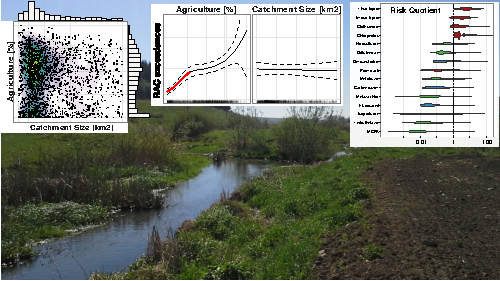
\includegraphics[width=0.7\textwidth]{abstract.pdf}

\end{tocentry}


%%%%%%%%%%%%%%%%%%%%%%%%%%%%%%%%%%%%%%%%%%%%%%%%%%%%%%%%%%%%%%%%%%%%%
\begin{abstract}
% 150-200 words
Small streams are important refugia for biodiversity.
In agricultural areas they may be at high risk from pesticide pollution. 
However, most related studies have been limited to a few streams on the regional level, hampering extrapolation to larger scales. We used data from german governmental water quality monitoring to quantify the drivers of pesticide exposure and to assess pesticide risk in small streams on a large scale. The data set comprised of 2,918,604 measurements related to 42,236 samples in 3,049 sampling sites and of 484 pesticides. We investigated the influence of agricultural land use, catchment size, as well as precipitation and seasonal dynamics on pesticide exposure using new statistical modeling techniques that explicitly  consider the limit of quantification. 
\newline
\begin{itshape} die naechsten 2 Saetze sind noch schwach - hier muessen auch Zahlen hin - ausserdem sollten die Risiken klarer dargestellt werden inklusive der verantwortlichen Substanzen
\end{itshape}
\newline
Agriculture land use lead to an xxx-fold increase in xxx once the proportion of agriculture in a catchment exceeded yyy.
Precipitation during and before sampling increased measured pesticide concentrations xxx-fold. The highest concentrations were found during summer, though this varied with compound. Risk thresholds were exceeded in yyy percent of streams, with neonicotinoid and other insecticides exhibiting highest frequencies of exceedance. We conclude that pesticides from agricultural land use are a major threat to small streams and their biodiversity, and that governmental pesticide sampling should be adapted to precipitation events in summer.
\newline
\begin{itshape} oder irgendsowas - auf jeden Fall irgendwas spektakulaerers als zu sagen dass pestizide ein risiko darstellen, dass ist nicht sonderlich neu
\end{itshape}

% Total words: 199
\end{abstract}


%% -------------------------------------------------------------------------
\section{Introduction}
More than 50\% of the total land area in Germany is used by agriculture \citep{statistisches_bundesamt_bodenflache_2014}.
In the year 2014 more than 45,000 tonnes of 766 authorized pesticides were sold for application on this area \citep{bundesamt_fur_verbraucherschutz_und_lebensmittelsicherheit_absatz_2015}.
The applied pesticides may enter surface waters via spray-drift, edge-off-field run-off or drainage \citep{stehle_probabilistic_2013,schulz_comparison_2001,liess_determination_1999}.
Once entered the surface waters they may have adverse effects on biota and ecosystem functioning \citep{schafer_thresholds_2012}. 
Although it is known that pesticide pollution and its ecological effects increase with the fraction of agricultural land use in the catchment \citep{schulz_field_2004}, the shape of the relationship is unknown and studies on potential thresholds are lacking.

Two recent studies indicate that pesticides might threaten freshwater biodiversity in the European union. 
\citet{malaj_organic_2014} analyzed data supplied to the European Union (EU) in the context of the Water Framework Directive (WFD) and showed that almost half of European water bodies are at risk from pesticides.
\citet{stehle_pesticide_2015} compiled 1,566 measured concentrations of 23 insecticides in the EU from scientific publications. 
They found that many of these measurements exceed regulatory acceptable concentrations (RAC). 
However, these studies reflect only a small amount of potentially available data (173 sites in predominantly mid-sized and large rivers in \citet{malaj_organic_2014} and 138 measurements in \citet{stehle_pesticide_2015}), and it is unclear how representative they are for Germany. %173 see Schäfer et al. 2016, Stehle: Table 2. 
Much more comprehensive data on thousands of sites are available from national monitoring programs that are setup for the surveillance of water quality, which is done independently by the federal states in Germany in compliance with the WFD \citep{quevauviller_water_2008} and additional state specific needs. 
Despite these data providing the opportunity to study pesticide risks and other research questions on a large scale with high spatial density, to date these data have not been compiled and related analyses are lacking.

Small water bodies (SWB) comprise a major fraction of streams \citep{nadeau_hydrological_2007}
%needs a definition here!
, accommodate a higher proportion of biodiversity compared to larger freshwater systems \citep{davies_comparison_2008, biggs_report_2014} and play an important role in recolonization of disturbed downstream reaches \citep{liess_analyzing_2005, orlinskiy_forested_2015}.
However, SWB might be also at high risk of pesticide contamination from adjacent agricultural areas and lower dilution potential \citep{schulz_field_2004,liess_determination_1999}.
Indeed, meta-analyses using data from studies with a few sites reported higher pesticide pollution in smaller streams compared to bigger streams \citep{stehle_pesticide_2015,schulz_field_2004}.
Despite their ecological relevance and potentially higher pesticide exposure, a recent analysis of pesticide studies showed that a disproportionally small fraction of studies were conducted in SWB, and these were largely limited to a few sites \citep{lorenz_specifics_2016}. Consequently, knowledge on the pesticide pollution of SWB on larger scales is scant.

In this study we compiled and analyzed large scale chemical monitoring data from SWB in Germany. First, we analysed the shape of the relationship between pesticide risk, agricultural land use and catchment size and examined whether related thresholds for pesticide risks can be derived. Second, we investigated the influence of precipitation and seasonal dynamics on pesticide detections, given that precipitation proved an important driver of pesticide exposure in several small scale studies \citep{wittmer_significance_2010}\citep{schulz_field_2004}, but it is unknown whether a precipitation signal prevails on large scales. 
Finally, we quantified the current risks from pesticides in SWB in Germany.



%% -------------------------------------------------------------------------
\section{Methods}
\subsection{Data compilation}
We compiled pesticide monitoring data from sampling sites in streams with catchment sizes $\mathrm{< 150km^2}$ for the years 2005 to 2015 from all 13 non-city federal states of Germany (see Supplemental Table~S1 for the abbreviations of federal state names). 
% 150 km2 needs justification - can perhaps be linked to introduction, see comment above
We homogenized and unified all data provided by the federal states into a database and implemented a robust data cleaning workflow (see Supplemental Figure~S1 for details) \citep{poisot_best_2015}.

We identified chemical samples taken during heavy rainfall events by spatio-temporal intersection of sampling events with gridded daily precipitation data available from the German Weather service (DWD).
This data spatially interpolates daily precipitation values from local weather stations \citep{rauthe_central_2013}. 
We performed the intersection for the actual sampling date and the day before, to identify rain events during and up to 48 hours before sampling.
%details required - what is a heavy rainfall event, resolution of data. One question with such data is from which precipitation value increases in concentrations are detectable. Also interesting and may be added as question in the introduction

\subsection{Characterization of catchments}
We compiled a total of 3,049 sampling sites with pesticide measurements.
We delineated catchments upstream for each of the sampling sites using a digital elevation model (DEM) \citep{eea_digital_2013} and the multiple flow direction algorithm \citep{holmgren_multiple_1994} as implemented in GRASS GIS 7 \citep{neteler_grass_2012}.
Catchment delineation was manually checked for accuracy by comparison with state stream networks.
Given that the delineated catchments were accurate only for 30\% of the sites,
%a reviewer might ask how accuracy was defined/cehcked
we compiled complementary catchment size data from authorities that provided catchments for an additional (60\% of sites). Ten \% of sites lacked catchment size data and were omitted from the operations outlined below.

For each catchment we calculated the relative cover (in \%) with agricultural area based on Official Topographical Cartographic Information System (ATKIS) of the land survey authorities \citep{adv_atkis_2016}.
%it may be worth mentioning, what agricultural land cover is
Additionally, we used agricultural cover data provided by authorities (19\% of sites). 
For 78\% of the sites both, the proportion of agricultural land use and catchment size were available.
% see do_overview.R for numbers
% this section is puzzling - if you have 90% catchments, why is it only 78% in the end? It is also unclear what is the ATKIS coverage and why additional state-wide??? cover data was used...

A clear definition of SWB in terms of catchment or stream size is currently lacking \citep{lorenz_specifics_2016}. 
The WFD defines SWB with a catchment size between 10 and 100 km\textsuperscript{2}, without further categorisation of streams \textless 10km\textsuperscript{2}. 
\citet{lorenz_specifics_2016} defines SWB with catchment size \textless 10km\textsuperscript{2} as SWB.
Because of data scarcity of streams \textless 10~km\textsuperscript{2} (Figure~\ref{fig:fig3}) we define in this study all streams below 25~km\textsuperscript{2} as SWB. This catchment size corresponds to a stream width of approximately 2~meters (see Supplemental Figure~S2).
% erstens muss diese definitionsfragen weiter nach oben, da schon über die SWB gesprochen wird. Zweitens braucht hier eigentlich keine Definition zu erfolgen - man kann eher untersuchen, ob es eine zusammmenhang zwischen belastung und catchment size gibt. War das nicht früher mal drinne. Dann könnte man auch in der Einleitung diskutieren, dass das ein weiteres Ziel der Arbeit war. Drittens wundert man sich, warum wir Gewässer < 150 analysieren, wenn wir als Definition hier 25 anlegen. 


\subsection{Characterization of pesticide pollution}
We characterised pesticide pollution using regulatory acceptable concentrations (RAC) \citep{brock_linking_2010}.
RACs are derived during pesticide authorization as part of the ecological risk assessment.
No unacceptable ecological effect are expected if the environmental concentration remains below this concentration. 
%state here sth. like: that Stehle and Schulz showed that RAC exceedances reflect a decrease in biodiversity and from this perspective are ecologically relevant indicators. Otherwise regulatory values may not be "real" trhesholds because politically influenced and this potential criticism should be taken ahead
The German Federal Environmental Agency (UBA) provided RACs for the 105 compounds with highest detection rates (Supplemental Table~S2). 
We expressed RACs as Risk Quotient (RQ):

\begin{equation}
RQ_i = \frac{C_i}{RAC_i}
\end{equation}

where $C_i$ is the concentration of a compound $i$ in a sample.


\subsection{Statistical analyses}
All data-processing and analyses were performed using R \citep{r_core_team_r:_2016}.
To display differences in the spectra of analyzed compounds between federal states we used Multidimensional Scaling (MDS) based on Jaccard dissimilarity in conjunction with complete linkage hierarchical clustering using the vegan package \citep{oksanen_vegan:_2016}.
We expected non-linear responses to agriculture and catchment size and therefore, used generalized additive models (GAM) to establish relationships \citep{fewster_analysis_2000}.
We modeled the number of RAC exceedances (RQ \textgreater 1) as:

\begin{align}
\begin{split}
  No_i \sim NB(\mu_i, \kappa) \\
  % E(No_i) = \mu_i~and~Var(No_i) = \mu_i + \frac{\mu_i^2}{\kappa} \\
  log(\mu_i)= \beta_0 + f_1(agri_i) + f_2(size_i) + log(n_i) \\
\end{split}
\end{align}

where $No_i$ is the observed number of exceedances at site $i$. 
% die normalen Leser werden SChwierigkeit haben, das zu verstehen, z.B. wo in der FOrmel überhaupt RQ > 1 auftaucht
We modeled $No_i$ as resulting from a negative binomial distribution ($NB$) with .....
The proportion of agriculture within the catchment ($agri_i$) and the catchment size of the site ($size_i$) were used as predictors of .... 
$f_1$ and $f_2$ are smoothing functions using penalized cubic regression splines \citep{wood_generalized_2006}.
The degree of smoothness was estimated using restricted maximum likelihood (REML) during model fitting process \citep{wood_fast_2011}.
The number of samples per site ($n_i$) was used as an offset to account for differences in sampling efforts (number of samplings and of analysed compounds) at a site and is equivalent to modeling the rate of exceedances. 
%bleibt unklar, wie beides sampling and compound spectrum in n eingeht
% beta 0 nicht erklärt - warum eigentlich 0 und nihct i, müssen alle den gleichen parameter haben - und macht es überhaupt sinn einen achsen-schnittpunkt ungleich 0 zu haben?
We used point-wise 95\% Confidence Intervals (CI) of the first derivative of the fitted smooth to check if there are regions of statistically significant changes.
GAMs were fitted using the mgcv package \citep{wood_fast_2011}.

While agricultural land use and catchment size vary only between sites, this is not the case for precipitation which changes also with time.
Therefore, we modeled the effects of precipitation in a separate model.
% begründung bleibt unklar - warum separates modell, denn im modell oben taucht weder raum noch hier zeit auf... Entscheidend ist doch auch, dass oben die Anzahl der RAC exdeendances und hier RQ Response variables sind
RQ and concentrations show a skewed distribution with an excess of zeros (no pesticides detected and quantified). 
Therefore, we modeled these as two processes 
% das gleiche hätte man oben auch shcon erklären können?
(one generating values below the limit of quantification (LOQ) and one generating values above LOQ) using a Zero-Adjusted Gamma (ZAGA) distribution \cite{rigby_generalized_2005,stasinopoulos_gamlss.dist:_2016}:

\begin{align}
RQ_i \sim ZAGA(\mu_i, \sigma, \nu_i) = 
  \begin{cases}
    (1 - \nu_i)   & \quad  \text{if } y < LOQ \\
    \nu_i \times f_{Gamma} (\mu_i, \sigma) & \quad \text{if } y \ge LOQ \\
  \end{cases}
  \label{eqn:eqn3}
\end{align}

$\nu_i$ denotes the probability of an observation i being above LOQ and $f_{Gamma}$ denotes the gamma function and is used for values equal to or greater LOQ, with $\mu$ being the mean and $\sigma$ the standard deviation.
%weiß nicht, ob der normale leser kapiert, dass das mean und sd von RQ sind...
We used the $log(x+0.05)$ transformed precipitation at sampling date ($log~prec_0$) and the day before ($log~prec_{-1}$), as well as quarters of the year ($Q1-Q4$) as linear predictors for $\mu$ and $\nu$. 
We used appropriate link functions for $\mu$ and $\nu$ and assumed $\sigma$ to be constant. 
Equation~\ref{eqn:eqn4} summarises the deterministic part of the model.

\begin{align}
\begin{split}
\log(\mu_{i}) = log~prec_{0 i} + log~prec_{-1 i} + Q1_{i} + Q2_{i}+Q3_{i}+Q4_{i}\\
logit(\nu_{i}) = log~prec_{0 i} + log~prec_{-1 i} + Q1_{i} + Q2_{i}+Q3_{i}+Q4_{i}
\end{split}
\label{eqn:eqn4}
\end{align}

To account for temporal auto-correlation and differences between federal states we used $site$ nested within $state$ as random intercepts.
Changes on $\mu$ can be interpreted as changes in the mean value of RQ, whereas changes in $\nu$ can be interpreted as changes in the probability of exceeding LOQ and showing any risk. 
%siehe oben - information könnte früher kommen
We implemented this model using the gamlss package \cite{stasinopoulos_generalized_2007}.

We fitted this model to each compound with a RAC, measured in least 1000 samples and with more than 5\% of values above LOQ (n = 24 compounds, see Supplemental Table~S3 for a list of compounds). 
To summarise the coefficients across the modeled compounds we used a random effect meta-analysis \citep{harrison_getting_2011}.
%müsste man vielleihct noch 2-3 sätze anfügen, was da genau gemacht wurde




%% -------------------------------------------------------------------------
\section{Results}
\subsection{Overview of the compiled data}


The compiled dataset used in analysis comprised 2,918,604 pesticide measurements of 42,236 samples in 3,049 sampling sites.  %see do_overview.R for numbers.
These samples were taken via grab sampling.  % see clean.R for numbers
Composite samples of different durations that were taken in 33 sites were not considered in analysis, given a potential methodical bias and the low sample size.
We found large differences in the number of sampling sites between federal states and their spatial distribution (Figure~\ref{fig:fig1} and Supplemental Table~S1).
% ein kritischer reviewer wird hier nachfragen: Wie repräsentativ für deutschland ist das dann. Ferner sollte man Erklärungen liefern warum MV und NI, Saarbrücken kaum Probestellen haben und weiß nicht, ob man die überhaupt reinnehmen sollte z.B. in Figure 2. Lässt sich doch schwer behaupten, dass Niedersachsen ein anderes Spektrum hat, wenn man 2 Stellen mit 500 eines anderen Bundeslandes vergleicht. INsgesamt wird auch nicht erwähnt, dass wir nur Stellen kleiner 100 abgefragt haben?! Das müsste vielleicht noch irgendwo erwähnt werden

\begin{figure}[ht]
  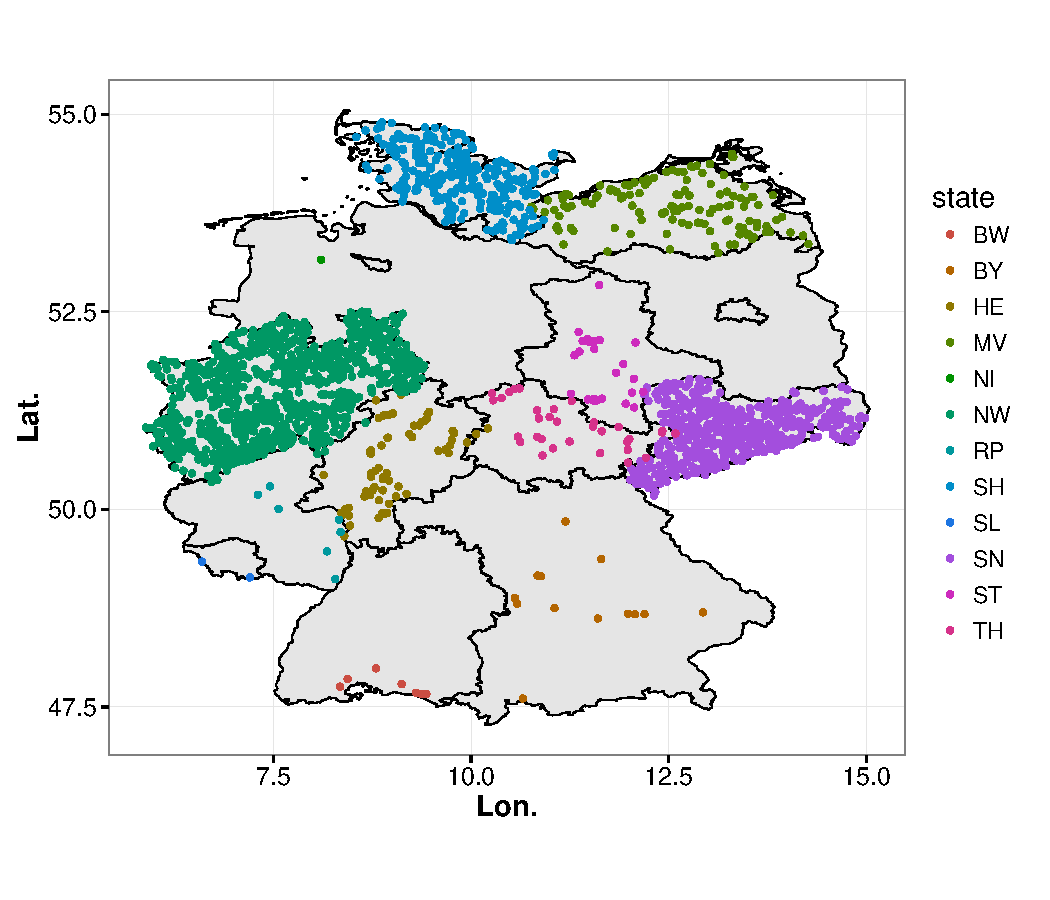
\includegraphics[width=0.6\textwidth]{figure1.pdf}
  \caption{Spatial distribution of the 3109 sampling sites. Colour codes different federal states, see Supplemental Table~S1 for abbreviations.}
  \label{fig:fig1}
\end{figure}

In total 484 different compounds used as pesticides and their metabolites were measured at least once (Supplemental Table~S2). 
Most of the compounds were herbicides (179), followed by insecticides (117) and fungicides (109).
Most samples were taken in the months April till October, with fewer samples during winter (see Supplemental Figure~S3).
Only 5.5\% (160,800) of all measurements were detects above the limit of quantification (LOQ).
We found substantial differences in the spectra of analyzed compounds between federal states (Figure~\ref{fig:fig2}).
Hierarchical clustering revealed three groups (see also Supplemental Figure~ S4):

\begin{enumerate}[i)]
	\item with less than 100 compounds (SL, ST and TH)
	\item with medium sized spectra
	\item with a big and distinct spectrum (RP and NI)
\end{enumerate}
% bei i ist eine zahl gegeben, kann man das für ii un iii auch machen? Was medium und big ist, ist ja recht subjektiv
\begin{figure}[ht]
  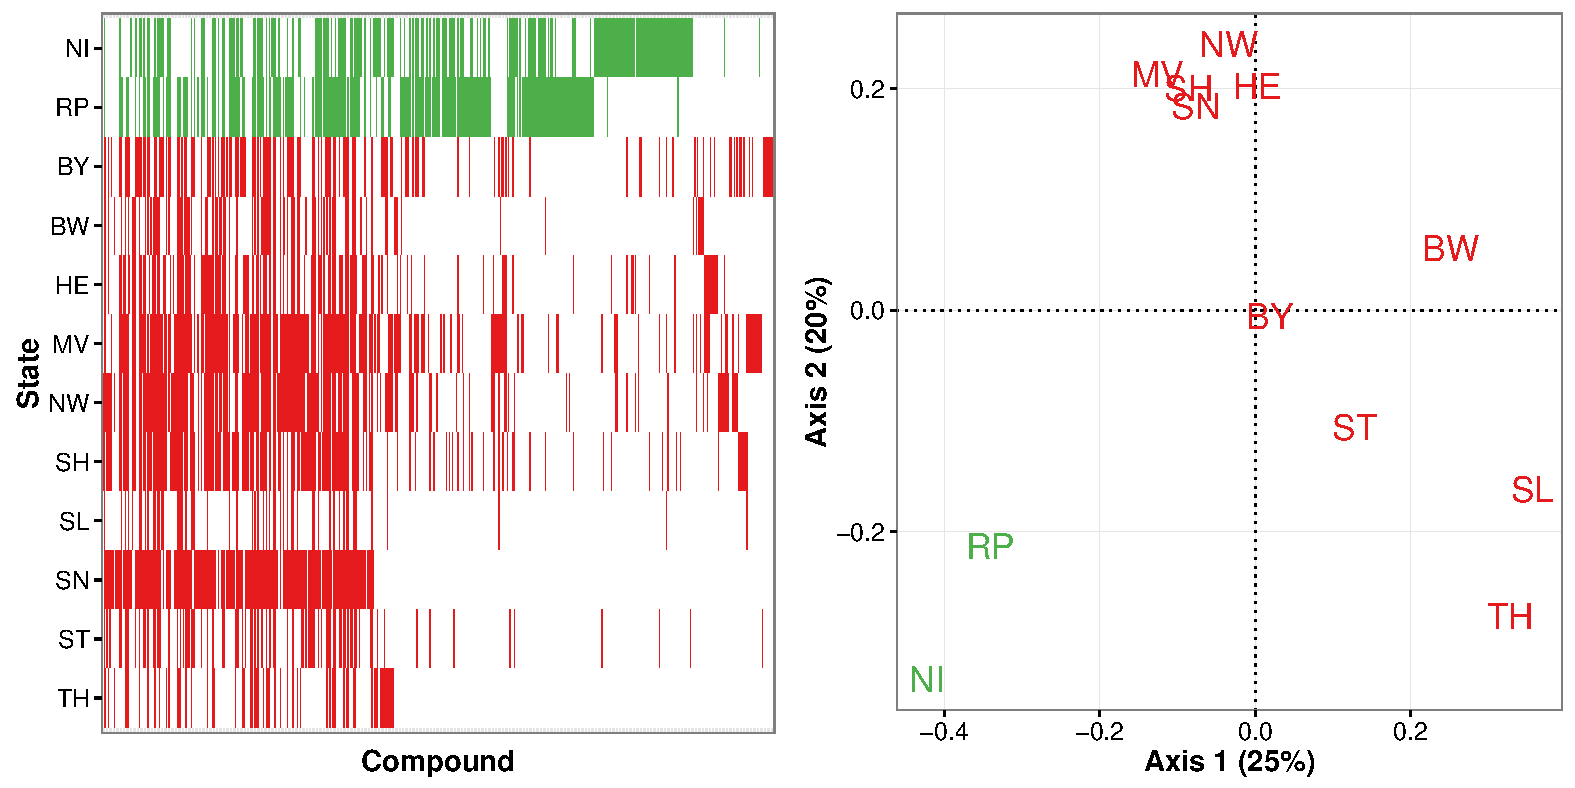
\includegraphics[width=\textwidth]{figure2.pdf}
  \caption{Compound spectra of the different federal states. Left: Barcode plot - each vertical line is an analysed compound. Right: MDS ordination. 
  Colors according to three groups determined by hierarchical clustering (see Supplemental Figure~S4).}
  \label{fig:fig2}
\end{figure}

The distribution of sampling sites across catchment sizes indicated a disproportionally low number of sites in catchments below $10~km^2$, with most sampling sites in catchments between 10 and 25 $km^2$ (Figure~\ref{fig:fig3}).
% vielleicht müsste man irgendwo nochmal schreiben, dass die zahl der kleinen gewässer zunimmt und man eben diese abnahme sieht in der verteilung
The proportion of agriculture in the catchments tended to decrease with increasing catchment size.
% put a statement here like: For example, only x% of sites had more than 75% agriculture in catchments larger 100 km2, whereas in catchments below 100 km2, yyy% of sites had more than 75% agriculture in their catchment.

\begin{figure}[ht]
  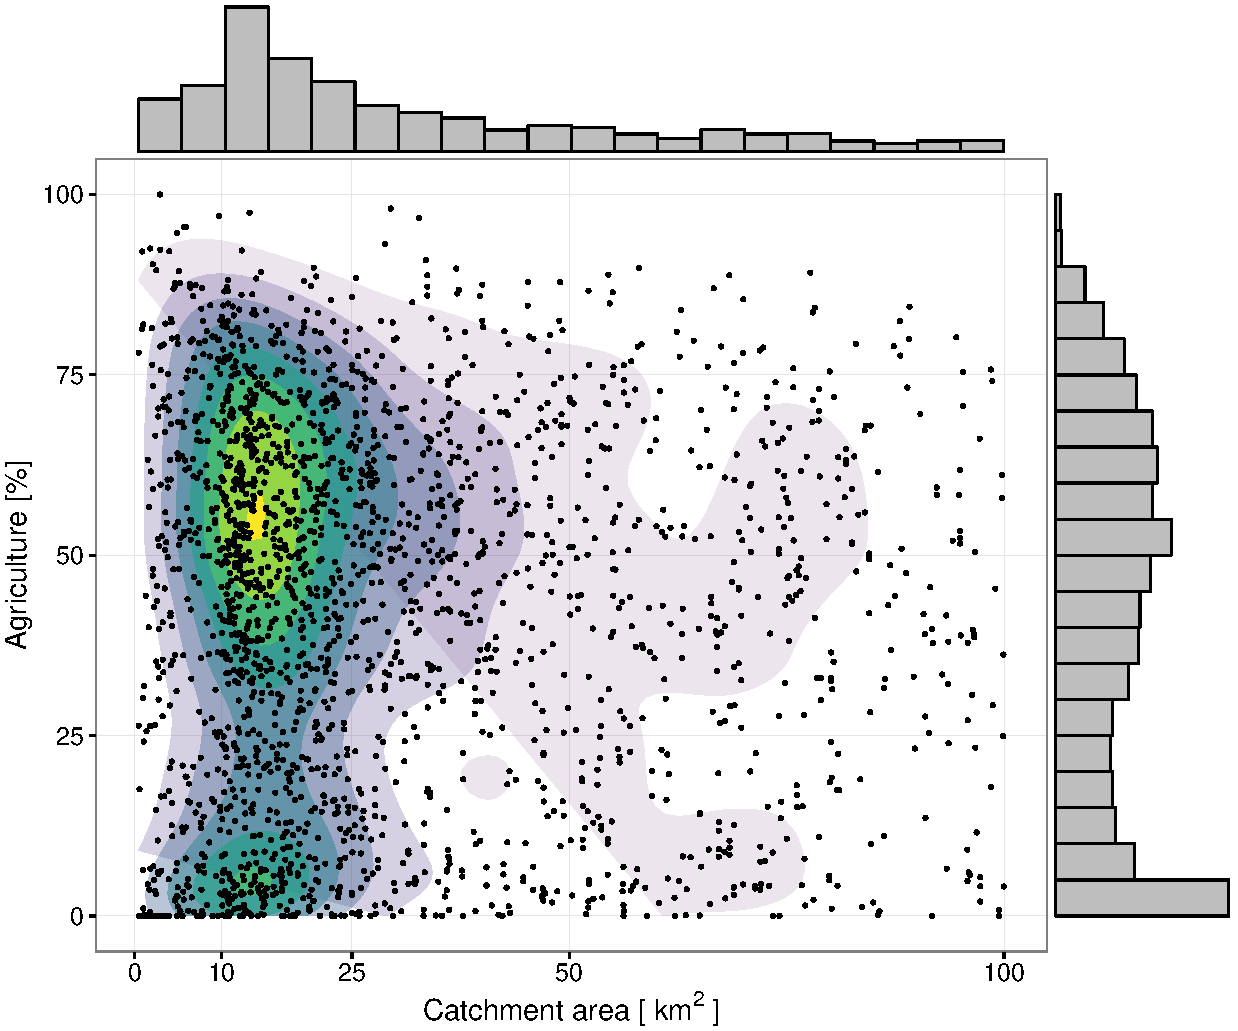
\includegraphics[width=.8\textwidth]{figure3.pdf}
  \caption{Distribution of catchment area and agriculture within the catchment area across the sampling sites.
  Only sampling sites with catchment area < 150 km\textsuperscript{2} are displayed. 
  Colour codes the 2-dimensional density of points.}
  \label{fig:fig3}
\end{figure}


\subsection{Influence of agricultural land use and catchment size}
The number of RAC exceedances increased strongly and statistically significant up to 25\% agriculture within the catchment.
Above this threshold the exceedances levelled followed by an increase above 75\% (Figure~\ref{fig:fig4}, left).
Catchment size had no statistically significant effect on the number of RAC exceedances (Figure~\ref{fig:fig4}, right).
We also found no statistically significant interaction between catchment size and agriculture.

\begin{figure}[ht]
  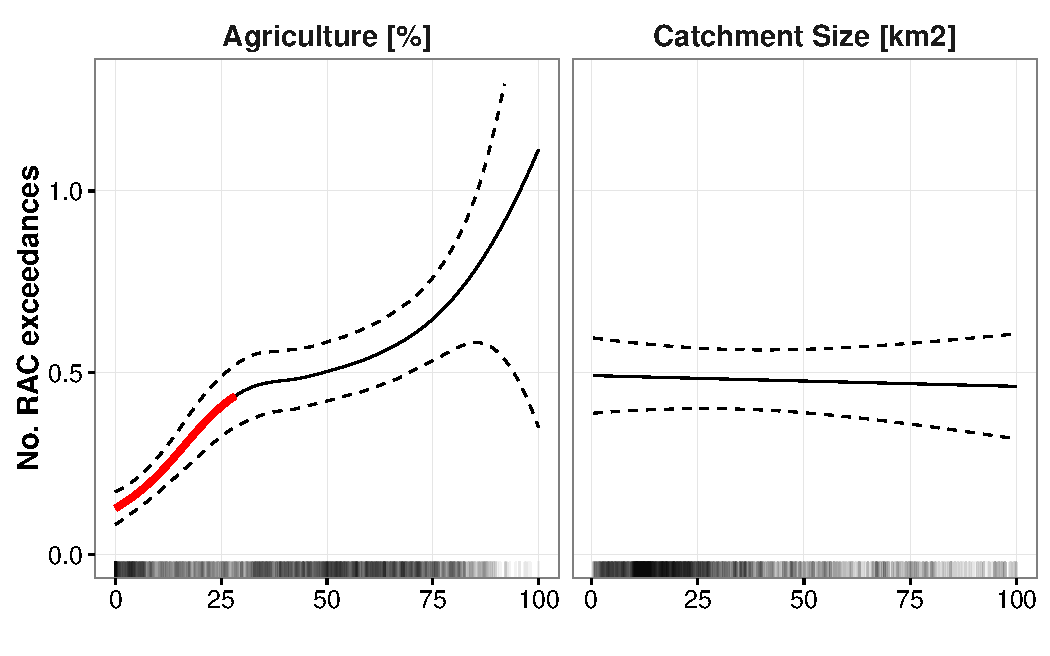
\includegraphics[width=0.95\textwidth]{figure4.pdf}
  \caption{Effect of \% agriculture within the catchment (left) and catchment size (right) on the number of RAC exceedances. Red line marks statistically significant changes. Dashed lines denote 95\% point-wise Confidence Intervals.
  }
  \label{fig:fig4}
\end{figure}


\subsection{Effect of precipitation on pesticide exposure}
The spatio-temporal intersection revealed that 5\% of the samples were taken at or after days with rainfall events greater than 10mm / day (Supplemental Figure~S6).
%warum hier die 10 mm, oben scheint es so, als wenn einfach die menge modelliert wurde und dann bekommt man ja auch eher raus, wie der einfluss der precipitation ist...
$prec_{0}$ and $prec_{-1}$ increased the probability of exceeding LOQ and the mean value of RQ.
Precipitation before sampling ($prec_{-1}$) had a stronger effect than precipitation during sampling ($prec_{0}$). 
This difference was less pronounced for the mean value of RQ (Figure~\ref{fig:fig5}, top).
% wäre vielleicht auch nicht schlecht einen satz zur interpretation der parameter zu geben: z.B. each increase of 10 mm in precipitation corresponded to an increase in ... of ...
The first quarter showed the lowest RQ and probability of exceeding LOQ.
Both increased during summer months and decreased towards the end of the year.
The differences were less pronounced for the mean value RQ and with higher variation (Figure~\ref{fig:fig5}, bottom).


\begin{figure}[ht]
  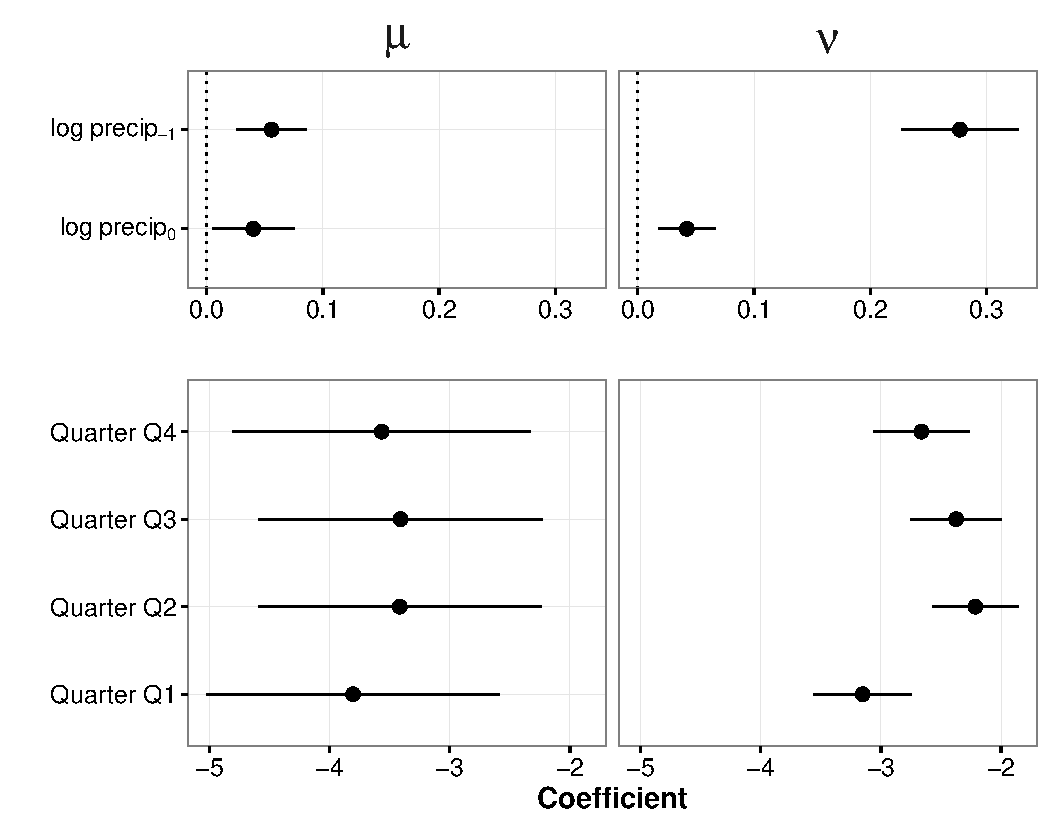
\includegraphics[width=0.8\textwidth]{figure5.pdf}
  \caption{Summarised coefficients (and their 95\% CI) for precipitation (top row) and quarter (bottom row) from a meta-anaylsis of the 24 modeled compounds. Left column: coefficients for mean RQ ($\mu$), right column: coefficients for probabilty to exceeed LOQ ($\nu$). 
  Coefficients are shown on the link scale (see Eq.~\ref{eqn:eqn4}).
  Single compound coefficients are provided in the Supplemental Table~S4 and Figure~S7).
  }
  \label{fig:fig5}
\end{figure}



\subsection{Pesticides in small water bodies}
% man kann sich natürlich fragen, warum hier der datensatz reduziert wird, wenn catchment size eh kaum einfluss hat. dafür braucht es oben eine gute begründung. auch warum alle analysen mit dem vollen datensatz gemacht werden, außer dieser
The dataset comprised 12,710 samples from 1,295 small water bodies.
In 1,173 samples (0.3\% of all and 5.6\% of samples with detects) RQ higher than 1 were observed.
Neonicotinoid insecticides and Chlorpyrifos showed the highest RQ exceedances (Figure~\ref{fig:fig6}).
For Thiacloprid, Imidacloprid and Chlorpyrifos the RAC was less than LOQ, therefore, all detections have a RQ~\textgreater~1. 
The herbicides Nicosulfuron and Diflufenican, as well as the fungicide Dimoxystrobin also showed high exceedances of RQ (29.5, 14.2 and 21.4 \% of all samples with detects).
The highest RQ were observed for Chlorpyrifos (max(RQ) = 244), Dimoxystrobin(max(RQ) = 117) and Isoproturon (max(RQ) = 80). 
Where analysed, metabolites exhibited the highest detection rates (for example, Metazachlor sulfonic acid was detected in 82\% of all samples were it was analysed, see also Supplemental Figure~S9).
Glyphosate was the compound with the highest detection rates, followed by Boscalid and Isoproturon. 
However, only the latter showed RQ exceedances (Figure~\ref{fig:fig6}).
In 44.8\% of samples more than one compound was quantified, with a maximum of 54 different compounds in one sample (Supplemental Figure~S8). 
%exceedances per site sollten hier erwähnt werden, nicht erst in Diskussion

\begin{figure}[ht]
  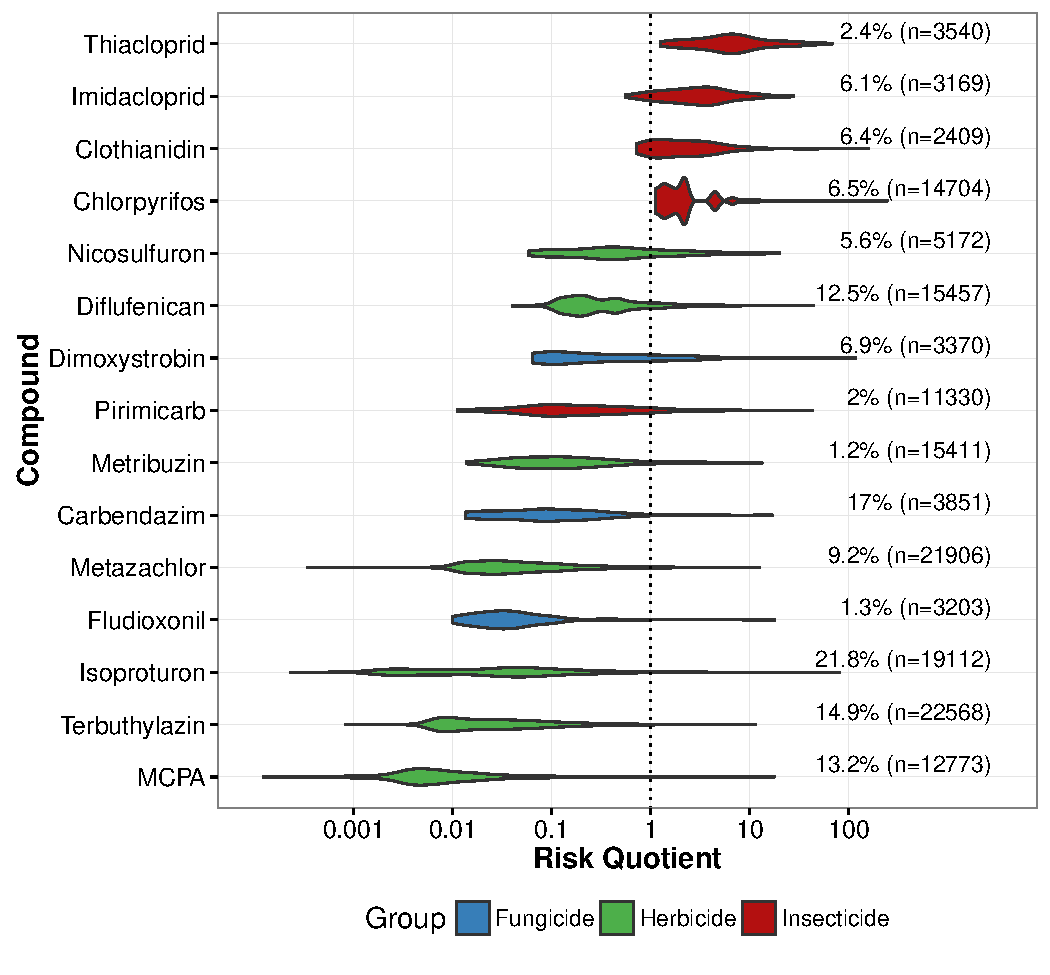
\includegraphics[width=0.6\textwidth]{figure6.pdf}
  \caption{15 compounds with the highest risk quotients in SWB. Non-detects are not shown due to the logarithmic axis. Numbers on the right give the percentage of values \textgreater LOQ and the total number of samples were the compound was analysed.
  }
  \label{fig:fig6}
\end{figure}




%% -------------------------------------------------------------------------
\section{Discussion}
\subsection{Overview on the compiled dataset}
The compiled dataset of governmental monitoring data represents currently the most comprehensive one available for Germany.
Similar nationwide datasets have been compiled for the Netherlands \citep{vijver_spatial_2008}, Switzerland \citep{munz_pestizidmessungen_2011} and the United States (Water Quality Portal (WQP) \url{www.waterqualitydata.us}).
The data compiled and analysed here for Germany is of similar quantity and quality.

% current problems in monitoring and possible solutions
Nevertheless, a nationwide assessment of pesticide pollution is hampered by the inhomogeneity of monitoring data between federal states:
There are not only big differences in the spatial distribution and quantity of sampling sites (Figure~\ref{fig:fig1}), but also the spectrum of analyzed compounds (Figure~\ref{fig:fig2}) and differences in the quality of chemical analyses. 
For Thiacloprid, Imidaclorpid and Chlorpyrifos LOQ were above RAC.
For these compounds a lowering of LOQ is essential for reliable assessment.
Moreover, would a nation-wide assessment benefit from a harmonized spectrum of analysed compounds between federal states.

Given their high abundance in the landscape \citep{nadeau_hydrological_2007} SWB are underrepresented in the current monitoring (Figure~\ref{fig:fig3}). 
Especially, streams below 10~km\textsuperscript{2} are missing, which could be attributed to the missing categorisation in the WFD. 



\subsection{Influence of agricultural land use and catchment size}
% agriculture
We found a strong influence of agriculture on the pollution of streams.
If there is more the 25\% agriculture within a catchment pesticides, it is likely that RAC will be exceeded with an increase in fully agricultural catchments (above 75 \% agriculture).
To our knowledge this is the first study investigating such thresholds of pesticide exposure.
Thresholds for agricultural land use have only been investigated in the past for biological communities.
\citet{feld_response_2013} found change points of biological community metric for agricultural land use at 40\% in low lands. 
Similarly, \citet{waite_agricultural_2014} found a threshold for aquatic diatoms at 40\%.
Our results coincide with these thresholds and suggest that pesticides might contribute to the observed biological changes. 

% size
We did not find a relationship between pesticide pollution and catchment size.
However, previous studies have shown that SWB are more polluted that bigger streams \citep{schulz_field_2004,stehle_pesticide_2015,knauer_pesticides_2016}.
This could be explained by the relatively short gradient of catchment sizes in our dataset, with most of the streams being \textless $100~km^2$ (Figure~\ref{fig:fig3}, top).
For example the gradient of \citet{schulz_field_2004} covered 6 orders of magnitude.
Another reason might be the unequal distribution of catchment sizes, with fewer sites below $10~km^2$ and above $100~km^2$ catchment size (Figure~\ref{fig:fig3}, top).



\subsection{Effect of precipitation on pesticide exposure}
Our results revealed that pesticide sampling for chemical monitoring in Germany is mainly performed when no precipitation occurs. 
Nevertheless, we found higher RQ if samples where taken after rainfall events. 
Samples taken at the day of a rainfall-event showed less risk, than samples taken one day after a rainfall-event.
This could be explained by a sampling just before the actual rainfall event.
Pesticide concentrations in agricultural SWB generally show short term peak concentrations \citep{wittmer_significance_2010}, therefore, a sampling at the day after a rainfall-event might miss peak concentrations.
The effects of precipitation were more pronounced for the probability to exceed LOQ, with smaller effect sizes for RQ.
This could be attributed to a higher variability of absolute concentrations.
Overall, our results indicate that current pesticide monitoring strongly underestimates pesticide exposure.
Automatic event-drive samplers \citep{stehle_probabilistic_2013} and passive samplers \citep{fernandez_calibration_2014,moschet_evaluation_2015} may help overcome these shortcomings and provide a better representation, especially for SWB \citep{lorenz_specifics_2016}. 

We found highest the probability of exceeding LOQ during summer (9.9\% for Q2) and lowest in the first Quarter (2.8\%, Figure~\ref{fig:fig5}, bottom right).
This yearly pattern coincides with their main application season for pesticides.
Nevertheless, there are compound specific differences in the yearly pattern, which explain the wide CI for the absolute RQ (Figure~\ref{fig:fig5}, bottom left).
For example, the herbicide Diflufenican showed highest RQ during the winter quarters (Supplemental Table~S4), which is the application period it is registered for in Germany \citep{bvl_online_2016}.
Our study suggest that pesticide exposure shows compound specific spatio-temporal dynamics.
Currently, little is known on these and further research on those might provide useful information for future ecological risk assessment. 


\subsection{Pesticides in small water bodies}
Our results suggest that SWB are frequently exposed to biologically relevant pesticide concentrations.
\citet{stehle_pesticide_2015} found the highest percentage of RAC exceedances for organophosphate insecticides. 
By contrast, our results revealed that neonicotinoid insecticides show high exceedances, followed by the organophosphate chlorpyrifos. 
This difference can be attributed to the low sample size for neonicotinoid insecticides in their study (n = 33) compared to the dataset presented here (between 1,290 and 2,113 samples in SWB, Figure~\ref{fig:fig6}). 
Our results shows that this particular class of insecticides may currently pose a high risk to freshwater ecosystems.
Compared to \citet{stehle_pesticide_2015} we found much lower rates RAC exceedances (0.3\% of 372,304 samples with RAC vs 44\% of 1,566 samples). 
This can be attributed to different aims of the data sources: scientific research aims at finding pollutants, whereas monitoring aims mainly at surveillance of water quality, also during periods with lower pesticide usage and at natural sites. 
Contrary, \citet{knauer_pesticides_2016} found exceedances from monitoring data mainly for herbicides and fungicides and only one insecticide Chlorpyrifos.
This might reflect differences in pesticide use between countries and defined RACs.

From the definition of RAC it follows that if the concentration of a compound exceeds its RAC ecological effects are expected.
Accordingly, \citet{stehle_agricultural_2015} found that biological diversity is significantly reduced at a RQ of 1.12.
We found RQ values greater than 1.12 at 25\% of all SWB sites. 
Consequently, we conclude that pesticides from agricultural land use are a major treat to small water bodies, the biodiversity they host and the services they provide. 
Additional treat arises when taking into account that most pesticides do not occur individually but in mixtures \cite{schreiner_pesticide_2016} and may co-occur with other stressors \citep{schafer_contribution_2016}.

% Approval / Risk Assessment
Monitoring data, despite the outlined limitations, provides an opportunity to study large scale environmental occurrences of pesticides.
Nevertheless, such nationwide compilations, may not only be used for governmental surveillance, but also to answer other questions, like validation of exposure modeling \cite{knabel_fungicide_2014}, retrospective evaluation of regulatory risk assessment \citep{knauer_pesticides_2016,stehle_pesticide_2015}or occurrences of pesticide mixtures \cite{schreiner_pesticide_2016}. 
The high exceedances of RAC indicate that the approval process for pesticides must be checked and refined.




%%%%%%%%%%%%%%%%%%%%%%%%%%%%%%%%%%%%%%%%%%%%%%%%%%%%%%%%%%%%%%%%%%%%%
\begin{acknowledgement}
The authors thank the federal state authorities for providing chemical monitoring data and the German Federal Environmental Protection Agency (UBA) for funding a related project (FKZ 3714 67 4040 / 1). 
\end{acknowledgement}


%%% Word count
% abstract    :  200
% 4 big(600)  : 2400
% 2 small(300):  600
% text body   : 3200
% ackno       :   24
% ======================================
% total       : 6424

%%%%%%%%%%%%%%%%%%%%%%%%%%%%%%%%%%%%%%%%%%%%%%%%%%%%%%%%%%%%%%%%%%%%%
\begin{suppinfo}
The following files are available free of charge.
\begin{itemize}
  \item Supplemental\_Materials.pdf : Supplemental Materials (Figures, Tables, Models).
\end{itemize}
\end{suppinfo}


%%%%%%%%%%%%%%%%%%%%%%%%%%%%%%%%%%%%%%%%%%%%%%%%%%%%%%%%%%%%%%%%%%%%%
\bibliography{references}

\end{document}
